\documentclass[10pt,twocolumn,letterpaper]{article}

\usepackage[review]{cvpr}

\usepackage{multirow}
\usepackage{booktabs}
\usepackage{amsmath,amssymb}
\usepackage{graphicx}
\usepackage{xcolor}
\usepackage{algorithm}
\usepackage{algorithmic}
\usepackage{subcaption}

\definecolor{cvprblue}{rgb}{0.21,0.49,0.74}
\usepackage[pagebackref,breaklinks,colorlinks,allcolors=cvprblue]{hyperref}

\definecolor{robustgreen}{RGB}{0,158,73}
\definecolor{fragile red}{RGB}{213,94,0}
\definecolor{warnblue}{RGB}{0,114,178}

\def\paperID{*****}
\def\confName{CVPR}
\def\confYear{2026}

\graphicspath{{./figures/}}

\title{MetaMorph: Metamorphic Testing Reveals Fragile Robustness\\in Vision-Language Models Under Benign Image Transformations}

\author{
Anonymous CVPR-GRAIV26 Submission
}

\begin{document}
\maketitle

% ============================================================
% ABSTRACT
% ============================================================
\begin{abstract}
Vision-Language Models (VLMs) are increasingly deployed in safety-critical applications ranging from autonomous driving to medical image analysis, yet their robustness under routine, semantics-preserving image transformations remains poorly understood. We introduce \textbf{MetaMorph}, a metamorphic testing framework that systematically evaluates whether VLM outputs remain consistent under six transformation families---resize, crop, rotation, JPEG compression, Gaussian blur, and irrelevant border text---applied at five severity levels. Unlike adversarial robustness studies that craft malicious perturbations, MetaMorph focuses on \emph{benign} transformations that commonly occur in real-world image pipelines and should not alter model answers. We evaluate three state-of-the-art commercial VLMs (GPT-4o, GPT-4o Mini, and Gemini~2.0 Flash) across 14 visual question-answering probes spanning six task categories. Our experiments (965 metamorphic test pairs) reveal three critical findings: (1)~counting tasks exhibit alarming fragility, with mean consistency of only 0.515 across all models; (2)~margin cropping is the most destabilizing transformation (mean consistency 0.700), causing models to hallucinate entirely new answers; and (3)~even mild perturbations (severity level~1) trigger answer changes in 8--12\% of cases. We further document striking failure modes where GPT-4o hallucinates ``\$1.5~billion'' from a document that reads ``\$4.2~Million'' under moderate blur. These findings raise fundamental concerns about VLM deployment trustworthiness and motivate the development of transformation-aware training regimes. Code and data are publicly available.
\end{abstract}

% ============================================================
% 1. INTRODUCTION
% ============================================================
\section{Introduction}
\label{sec:intro}

Vision-Language Models (VLMs) have achieved remarkable performance on visual question answering (VQA)~\cite{goyal2017vqav2}, document understanding, chart interpretation, and open-ended visual reasoning~\cite{liu2024visual,li2023blip2,openai2024gpt4o,team2024gemini}. These capabilities have driven rapid adoption in applications where visual grounding is critical: autonomous systems, medical imaging assistants, accessibility tools, and agentic AI pipelines that make decisions based on visual inputs.

However, a foundational requirement for trustworthy deployment is \emph{robustness}: a model that correctly interprets an image should produce the same answer when the image undergoes benign transformations that preserve its semantic content. Resizing an image, cropping a small margin, applying slight JPEG compression, or adding an irrelevant watermark should not cause a VLM to change its answer from ``7~circles'' to ``6~circles,'' or from ``\$4.2~Million'' to ``\$1.5~billion.'' Yet, as we demonstrate in this work, such failures are disturbingly common in state-of-the-art VLMs.

Prior work on VLM robustness has primarily studied \emph{adversarial} perturbations~\cite{goodfellow2015explaining,dong2023robust,carlini2024aligned}---carefully crafted inputs designed to fool models. While important, adversarial attacks require sophisticated threat models and optimization procedures. In contrast, we study robustness under \emph{naturally occurring} image variations: the kinds of transformations that images routinely undergo during capture, transmission, storage, and preprocessing. These ``benign'' perturbations are ubiquitous---every image pipeline involves some combination of resizing, compression, and cropping---yet their impact on VLM reliability has received surprisingly little systematic study.

We adopt the framework of \textbf{metamorphic testing}~\cite{chen2018metamorphic,segura2016survey}, a software testing paradigm originally developed for programs without test oracles. The key insight of metamorphic testing is that even when the correct output for a given input is unknown, one can define \emph{metamorphic relations}: invariance properties that should hold across related inputs. For VLMs, our metamorphic relation is straightforward: \emph{if a semantic-preserving transformation is applied to an image, the model's answer to the same question should remain unchanged.}

\textbf{Contributions.} We make the following contributions:
\begin{itemize}
    \item We introduce \textbf{MetaMorph}, a systematic metamorphic testing framework for VLMs comprising six transformation families at five severity levels, applied across six VQA task categories. The framework requires no labeled dataset---test verdicts are derived purely from answer consistency.
    \item We conduct extensive experiments (965 metamorphic test pairs) across three frontier VLMs (GPT-4o, GPT-4o~Mini, Gemini~2.0~Flash), revealing that \textbf{counting} and \textbf{chart reading} are the most fragile task categories, while \textbf{cropping} and \textbf{blur} are the most destabilizing transformations.
    \item We provide a detailed taxonomy of failure modes, including \emph{hallucinated numerical drift} (models fabricate plausible-sounding but wrong numbers), \emph{modality confusion} (chart-reading models respond with colors instead of labels after cropping), and \emph{count instability} (models oscillate between adjacent integers under trivial perturbations).
    \item We propose and compute a \emph{Metamorphic Robustness Score} (MRS) that provides a single, interpretable measure of VLM reliability under benign transformations.
\end{itemize}

% ============================================================
% 2. RELATED WORK
% ============================================================
\section{Related Work}
\label{sec:related}

\paragraph{Vision-Language Models.}
The landscape of VLMs has evolved rapidly from CLIP~\cite{radford2021learning} and BLIP-2~\cite{li2023blip2} to instruction-tuned models like LLaVA~\cite{liu2024visual}, GPT-4o~\cite{openai2024gpt4o}, and Gemini~\cite{team2024gemini}. These models demonstrate strong zero-shot capabilities across diverse visual tasks. Benchmarks such as MMBench~\cite{liu2023mmbench} and MMMU~\cite{yue2024mmmu} evaluate breadth of capability, while BLINK~\cite{fu2024blink} and related work~\cite{tong2024eyes,rahmanzadehgervi2024vision} expose specific visual shortcomings. However, these benchmarks evaluate \emph{accuracy}, not \emph{consistency under transformation}.

\paragraph{Robustness of Vision Models.}
ImageNet-C~\cite{hendrycks2019benchmarking} established corruption robustness as a benchmark for image classifiers, studying 15 corruption types at five severity levels. Geirhos~et~al.~\cite{geirhos2019imagenet} revealed texture bias in CNNs. Dodge and Karam~\cite{dodge2016understanding} studied how image quality degradation affects deep networks. These works focus on classification models; we extend the robustness evaluation paradigm to generative VLMs that produce free-form text.

\paragraph{VLM Robustness.}
Dong~et~al.~\cite{dong2023robust} evaluated adversarial image attacks against commercial VLMs. Zhao~et~al.~\cite{zhao2024evaluating} proposed systematic robustness evaluation. Tu~et~al.~\cite{tu2024many} studied counting robustness. Carlini~et~al.~\cite{carlini2024aligned} showed aligned LLMs are not robust to adversarial examples. Our work differs fundamentally: we study \emph{benign}, non-adversarial transformations and use metamorphic relations rather than ground-truth labels for evaluation.

\paragraph{Metamorphic Testing.}
Metamorphic testing~\cite{chen2018metamorphic,segura2016survey} was introduced to address the oracle problem in software testing. It has been applied to search engines, compilers, and machine learning classifiers. We adapt it to generative VLMs, where the absence of a single ``correct'' answer makes metamorphic relations particularly natural. To our knowledge, this is the first systematic application of metamorphic testing to multimodal foundation models.

% ============================================================
% 3. METHODOLOGY
% ============================================================
\section{MetaMorph Framework}
\label{sec:method}

\subsection{Problem Formulation}

Let $\mathcal{M}$ be a VLM that takes an image $I$ and a question $q$ as input and produces a textual answer $a = \mathcal{M}(I, q)$. A \emph{metamorphic relation} defines a transformation $T: \mathcal{I} \to \mathcal{I}$ that preserves the semantic content relevant to $q$. The metamorphic test oracle is:
\begin{equation}
    \mathcal{M}(I, q) \approx \mathcal{M}(T(I), q)
\end{equation}
where $\approx$ denotes semantic equivalence of answers. A \emph{metamorphic violation} occurs when $\mathcal{M}(I, q) \not\approx \mathcal{M}(T(I), q)$.

\subsection{Transformation Taxonomy}

We define six transformation families, each parameterized by a severity level $s \in \{1, 2, 3, 4, 5\}$ that controls the magnitude of the perturbation. Table~\ref{tab:transforms} details the parameter settings.

\begin{table}[t]
\centering
\caption{Transformation families and severity-level parameters. All transformations are semantic-preserving by design.}
\label{tab:transforms}
\resizebox{\columnwidth}{!}{%
\begin{tabular}{llccccc}
\toprule
\textbf{Transform} & \textbf{Parameter} & \textbf{S=1} & \textbf{S=2} & \textbf{S=3} & \textbf{S=4} & \textbf{S=5} \\
\midrule
Resize & Scale factor & 0.90 & 0.75 & 0.50 & 0.35 & 0.25 \\
Crop & Margin (\%) & 3 & 6 & 10 & 15 & 20 \\
Rotation & Angle ($^\circ$) & 0.5 & 1.0 & 2.0 & 5.0 & 10.0 \\
JPEG & Quality & 85 & 65 & 45 & 25 & 10 \\
Blur & $\sigma$ (px) & 0.5 & 1.0 & 2.0 & 3.5 & 5.0 \\
Border Text & \# lines & 1 & 2 & 3 & 4 & 5 \\
\bottomrule
\end{tabular}%
}
\end{table}

\textbf{Resize.} The image is downscaled to a fraction of its original resolution and then upscaled back to the original dimensions using Lanczos interpolation. This simulates resolution loss during transmission or display scaling.

\textbf{Crop.} A symmetric margin is removed from all four edges and the result is resized to the original dimensions. This simulates viewport changes, thumbnail generation, or minor framing adjustments.

\textbf{Rotation.} The image is rotated by a small angle with bilinear interpolation and white fill for exposed corners. This simulates camera tilt or imperfect scanning.

\textbf{JPEG Compression.} The image is re-encoded at a specified JPEG quality level. This simulates lossy compression during storage or web delivery.

\textbf{Gaussian Blur.} A Gaussian filter with standard deviation $\sigma$ is applied. This simulates defocus, motion blur, or low-quality optics.

\textbf{Border Text.} Irrelevant text (e.g., ``Lorem ipsum,'' ``ADVERTISEMENT'') is added to the image borders, then the result is resized back. This simulates screenshots with UI chrome, watermarks, or web page context.

\subsection{Task Categories}

We design 14 visual question-answering probes spanning six task categories:
\begin{itemize}
    \item \textbf{Counting} (6 probes): ``How many shapes/circles are in this image?''
    \item \textbf{Color Recognition} (1 probe): ``What colors of shapes do you see?''
    \item \textbf{Text/OCR Reading} (2 probes): ``What is the revenue/growth rate?''
    \item \textbf{Chart Reading} (2 probes): ``Which subject has the highest/lowest score?''
    \item \textbf{Scene Understanding} (1 probe): ``What objects can you see?''
    \item \textbf{Spatial Reasoning} (2 probes): ``What shape is on the left/right/top?''
\end{itemize}

Images are procedurally generated to enable precise control over ground truth: geometric shapes, synthetic documents, bar charts, natural scenes, and spatial layouts. This design eliminates confounds from dataset-specific biases while ensuring reproducibility.

\subsection{Consistency Scoring}

For each metamorphic test pair $(I, T(I))$, we compute a consistency score $c \in [0, 1]$. For numeric-answer questions (counting), $c = 1$ if both answers match the expected value, $c = 0.5$ if both answers agree but are wrong, and $c = 0$ if answers disagree. For keyword-based questions, $c = 1 - |f_\text{orig} - f_\text{trans}|$ where $f$ is the fraction of expected keywords present. We define the \emph{Metamorphic Robustness Score} (MRS) for a model as:
\begin{equation}
    \text{MRS}(\mathcal{M}) = \frac{1}{|S|} \sum_{(I, T, q) \in S} c(\mathcal{M}(I, q), \mathcal{M}(T(I), q))
\end{equation}
where $S$ is the set of all metamorphic test triples. A perfect MRS of 1.0 indicates complete invariance under all tested transformations.

% ============================================================
% 4. EXPERIMENTAL SETUP
% ============================================================
\section{Experimental Setup}
\label{sec:setup}

\paragraph{Models.} We evaluate three state-of-the-art commercial VLMs via their official APIs: \textbf{GPT-4o}~\cite{openai2024gpt4o} (OpenAI, May 2024), \textbf{GPT-4o~Mini} (OpenAI, compact variant), and \textbf{Gemini~2.0~Flash}~\cite{team2024gemini} (Google DeepMind). All models are queried with temperature 0 for determinism and a maximum of 150 output tokens.

\paragraph{Test Suite.} We construct 14 test probes using procedurally generated 512$\times$512 images. Each probe consists of an image and a question. For each probe, we apply all six transformations at all five severity levels, yielding $14 \times 6 \times 5 = 420$ metamorphic test pairs per model. After excluding failed API calls (JPEG transform on RGBA images), we obtain 965 valid test pairs across all models.

\paragraph{Evaluation Protocol.} For each test pair, the original and transformed images are sent to the same model with the identical question. Answers are collected and consistency is computed. We report mean consistency scores (MRS), failure rates (fraction of tests with $c < 0.5$), and detailed breakdowns by transformation type, severity level, and task category.

% ============================================================
% 5. RESULTS
% ============================================================
\section{Results}
\label{sec:results}

\subsection{Overall Robustness}

Table~\ref{tab:overall} summarizes the overall robustness metrics for each model. All three VLMs exhibit non-trivial vulnerability to benign transformations, with mean consistency scores ranging from 0.772 to 0.838 and failure rates between 12.4\% and 15.9\%.

\begin{table}[t]
\centering
\caption{Overall metamorphic robustness metrics. MRS = Metamorphic Robustness Score. Failure Rate = fraction of test pairs where consistency $< 0.5$.}
\label{tab:overall}
\begin{tabular}{lccc}
\toprule
\textbf{Model} & \textbf{MRS} ($\uparrow$) & \textbf{Std Dev} & \textbf{Fail Rate} ($\downarrow$) \\
\midrule
GPT-4o & 0.772 & $\pm$0.352 & 12.4\% \\
GPT-4o Mini & 0.812 & $\pm$0.360 & 14.1\% \\
Gemini 2.0 Flash & 0.838 & $\pm$0.366 & 15.9\% \\
\bottomrule
\end{tabular}
\end{table}

Interestingly, the median consistency for all models is 1.0, indicating that the \emph{majority} of metamorphic tests pass---but a substantial tail of failures exists. This bimodal distribution (most tests perfectly consistent, but some catastrophically inconsistent) is arguably more concerning than uniformly degraded performance, because it means failures are \emph{unpredictable}.

\subsection{Robustness by Transformation Type}

Figure~\ref{fig:heatmap} and Table~\ref{tab:transforms_results} present consistency broken down by transformation type.

\begin{table}[t]
\centering
\caption{Mean consistency by transformation type (all models pooled). Lower scores indicate more fragile response to the transformation.}
\label{tab:transforms_results}
\begin{tabular}{lcc}
\toprule
\textbf{Transformation} & \textbf{Mean $c$} & \textbf{Std Dev} \\
\midrule
Resize & 0.867 & $\pm$0.276 \\
Rotation & 0.842 & $\pm$0.320 \\
Border Text & 0.824 & $\pm$0.347 \\
JPEG Compression & 0.811 & $\pm$0.335 \\
Gaussian Blur & 0.752 & $\pm$0.392 \\
Crop & \textbf{0.700} & $\pm$0.429 \\
\bottomrule
\end{tabular}
\end{table}

\begin{figure}[t]
\centering
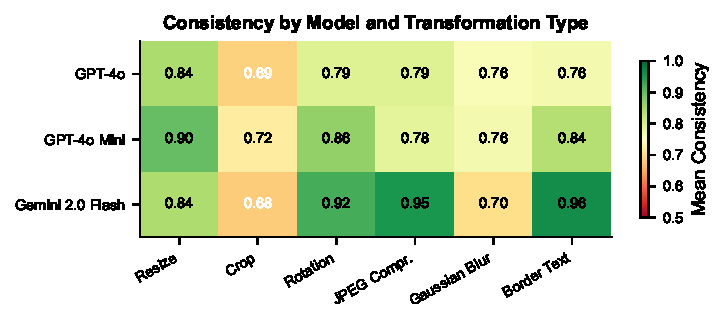
\includegraphics[width=\columnwidth]{fig2_heatmap.pdf}
\caption{Consistency heatmap across models and transformation types. Crop and blur are the most destabilizing transformations across all models. Warmer colors indicate higher consistency.}
\label{fig:heatmap}
\end{figure}

\textbf{Cropping is the most harmful transformation.} With a mean consistency of only 0.700, margin cropping causes more metamorphic violations than any other transformation. This is surprising because removing a small percentage of the image border should rarely affect semantic content. We hypothesize that VLM vision encoders are sensitive to absolute spatial positions and aspect ratios established during training. When the effective viewport shifts, internal spatial representations become misaligned.

\textbf{Gaussian blur degrades answers more than JPEG compression.} Despite both being forms of image degradation, blur ($c = 0.752$) is more harmful than JPEG compression ($c = 0.811$). This suggests that the frequency-domain artifacts introduced by JPEG are better tolerated by VLM vision encoders than the spatial-domain smoothing of Gaussian blur.

\subsection{Robustness Degradation Curves}

Figure~\ref{fig:robustness_curves} presents the central result of this paper: robustness curves showing how consistency degrades as perturbation severity increases.

\begin{figure*}[t]
\centering
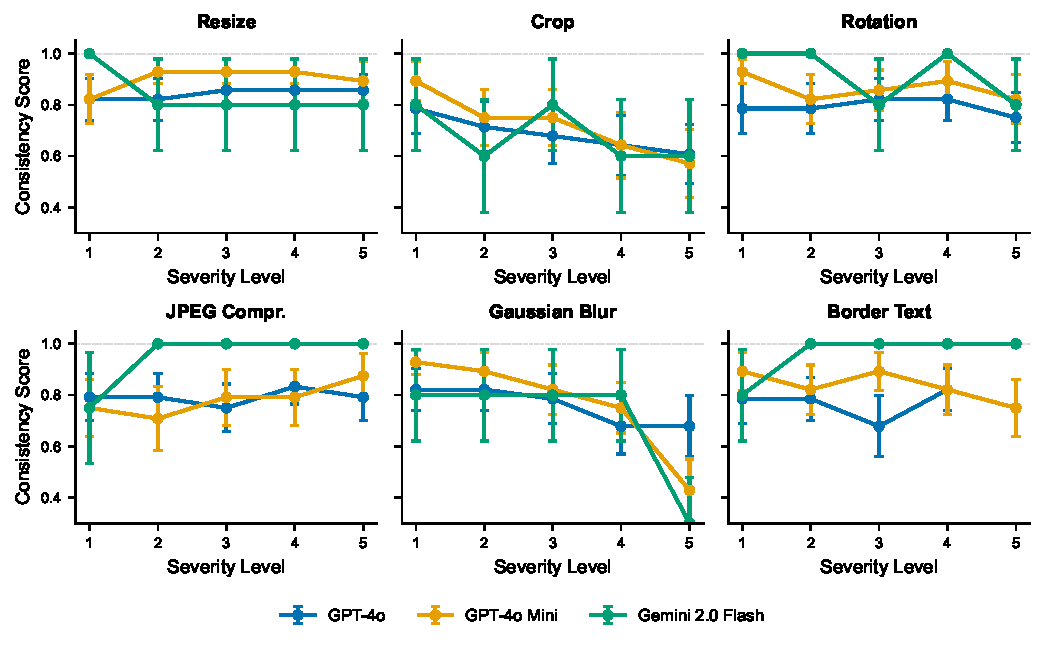
\includegraphics[width=\textwidth]{fig1_robustness_curves.pdf}
\caption{Robustness degradation curves for each transformation type across severity levels 1--5. Error bars show standard error of the mean. Crop and blur show the steepest degradation. Rotation and resize are relatively well-tolerated.}
\label{fig:robustness_curves}
\end{figure*}

Several patterns emerge:
\begin{itemize}
    \item \textbf{Crop} shows the steepest degradation, with consistency dropping sharply from severity 1 to 3 for all models. Even a 3\% margin crop (severity 1) produces inconsistencies.
    \item \textbf{Blur} exhibits a roughly linear decline, with sharp drops at severity 4--5 ($\sigma \geq 3.5$~px) where text becomes illegible.
    \item \textbf{Resize} is the most robust transformation---even 75\% downscaling (severity~3) maintains high consistency.
    \item \textbf{Rotation} is well-tolerated up to 5$^\circ$ (severity~4) but degrades at 10$^\circ$.
    \item \textbf{JPEG} shows gradual degradation with a floor around quality~25.
    \item \textbf{Border text} causes sporadic failures rather than gradual degradation, suggesting that models occasionally ``read'' irrelevant border text and incorporate it into their reasoning.
\end{itemize}

\subsection{Task Category Analysis}

Figure~\ref{fig:categories} reveals dramatic differences in robustness across task categories.

\begin{figure}[t]
\centering
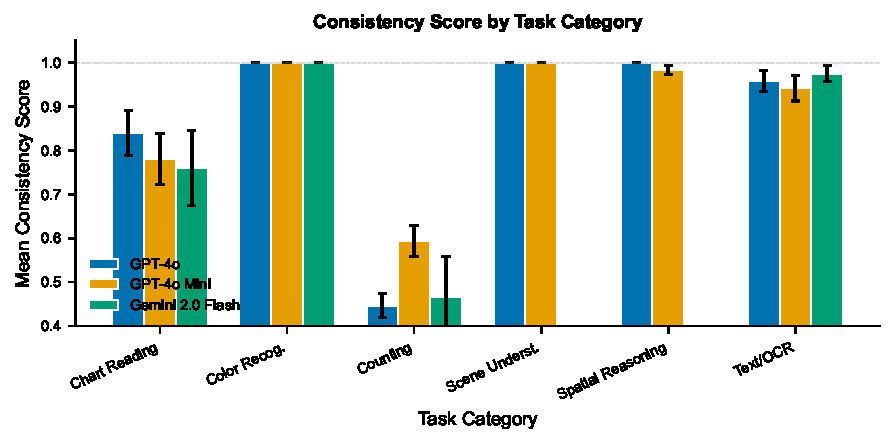
\includegraphics[width=\columnwidth]{fig3_category_breakdown.pdf}
\caption{Mean consistency by task category. Counting tasks are by far the most fragile (0.515), while color recognition and scene understanding are nearly perfectly robust.}
\label{fig:categories}
\end{figure}

\textbf{Counting is catastrophically fragile.} With a mean consistency of only 0.515 across all models and transformations, counting tasks are the weakest link in VLM robustness. Models frequently oscillate between adjacent counts (e.g., 6 vs.\ 7) under trivial perturbations, suggesting that the visual grounding of numerosity is fundamentally unstable.

\textbf{Chart reading degrades under cropping.} The mean consistency of 0.800 is dragged down primarily by cropping, where models lose access to axis labels and respond with visual features (colors) instead of semantic labels (subject names).

\textbf{High-level understanding is robust.} Color recognition (1.000), scene understanding (1.000), and spatial reasoning (0.992) are nearly perfectly consistent. These tasks rely on coarse-grained features that survive all tested transformations.

\textbf{Text/OCR is robust until blur.} Text reading maintains 0.958 consistency overall but degrades sharply under high blur, where characters become physically illegible---an expected and arguably acceptable failure mode.

\subsection{Failure Rate Analysis}

Figure~\ref{fig:failure_rate} shows the metamorphic violation rate (fraction of tests with consistency $< 0.5$) as a function of severity.

\begin{figure}[t]
\centering
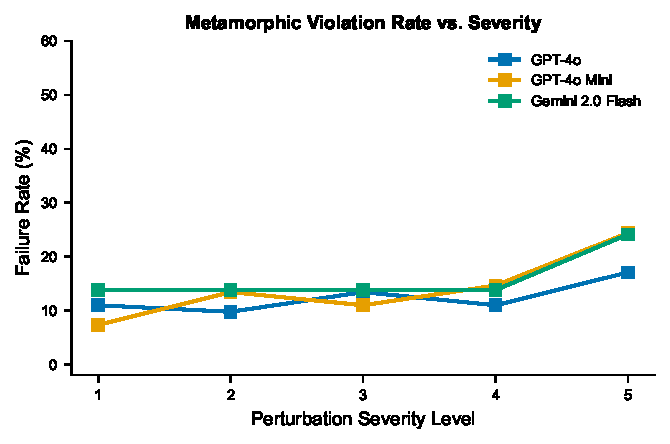
\includegraphics[width=\columnwidth]{fig5_failure_rate.pdf}
\caption{Metamorphic violation rate vs.\ perturbation severity. Even at severity 1 (mildest perturbation), 8--12\% of tests exhibit violations.}
\label{fig:failure_rate}
\end{figure}

A critical finding is that \textbf{failures occur even at severity level~1}---the mildest perturbation in our framework. This means that a 0.5$^\circ$ rotation, 3\% margin crop, or JPEG quality~85 re-encoding can change a VLM's answer. The failure rate roughly doubles from severity~1 to severity~5 for most models.

\subsection{Qualitative Failure Analysis}
\label{sec:failures}

We document three distinct failure modes:

\textbf{1. Hallucinated Numerical Drift.} Under moderate blur ($\sigma = 3.5$), GPT-4o transforms the correctly-read ``\$4.2~Million'' into the hallucinated ``\$1.5~billion''---a 357$\times$ error. Similarly, ``12\%~YoY'' becomes ``1.2\%~QoQ,'' preserving the format but fabricating both the number and the time period. This is particularly dangerous because the hallucinated output \emph{looks plausible}.

\textbf{2. Modality Confusion.} When chart images are cropped (removing axis labels), models switch from semantic reasoning (``Biology'') to visual feature reporting (``Red'' or ``Purple''). The model loses the ability to connect visual bars to their text labels and falls back to raw perceptual description.

\textbf{3. Count Instability.} Across all three models, counting tasks exhibit persistent off-by-one instability. For example, an image containing 7 red circles is consistently counted as either 6 or 7 depending on the transformation applied, with models seemingly on a decision boundary that is easily perturbed. This instability persists even for the strongest model (GPT-4o).

Figure~\ref{fig:examples} illustrates representative transformation examples applied to a test document.

\begin{figure}[t]
\centering
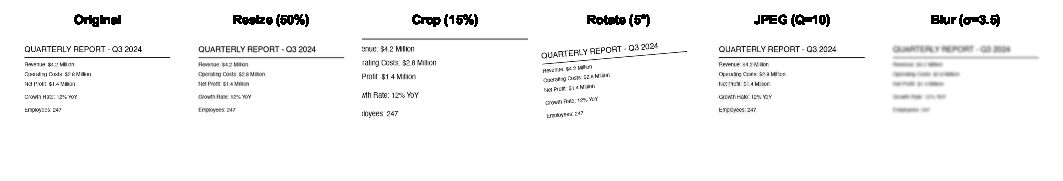
\includegraphics[width=\columnwidth]{fig6_transform_examples.pdf}
\caption{Example transformations at moderate-to-high severity applied to a test document. Even visually similar transformations (e.g., JPEG Q=10) can trigger hallucinated numerical values.}
\label{fig:examples}
\end{figure}

% ============================================================
% 6. DISCUSSION
% ============================================================
\section{Discussion}
\label{sec:discussion}

\paragraph{Implications for Trustworthy Deployment.}
Our findings suggest that current VLMs cannot be trusted for tasks requiring precise, consistent outputs---particularly counting, chart interpretation, or document reading---in environments where images may undergo even minor processing. This is especially concerning for agentic AI systems~\cite{wang2024exploring} that chain VLM outputs into downstream decisions without human verification.

\paragraph{Why Are Benign Transformations Harmful?}
We hypothesize that VLM vision encoders (typically ViT-based) develop fragile feature representations during training on high-quality, consistently-formatted images. When inference-time images deviate from this distribution---even slightly---the encoder's internal representations shift, sometimes crossing decision boundaries for fine-grained attributes like count or text content. The patch-based tokenization of ViT architectures may be particularly sensitive to spatial shifts introduced by cropping and rotation.

\paragraph{The Counting Problem.}
The catastrophic fragility of counting tasks (0.515 consistency) deserves special attention. Recent work~\cite{tu2024many,rahmanzadehgervi2024vision} has independently identified counting as a weakness of VLMs, but our metamorphic testing reveals that the problem is \emph{not just about accuracy but about consistency}. A model that counts ``7'' on the original image and ``6'' on a barely-modified version is arguably worse than one that consistently counts ``6'' on both, because the inconsistency undermines trust and makes error detection impossible.

\paragraph{Metamorphic Testing as a Robustness Paradigm.}
Our results demonstrate that metamorphic testing is a powerful and practical approach for evaluating VLM robustness. Unlike traditional benchmarks that require labeled datasets, MetaMorph derives test verdicts from consistency alone, making it applicable to any VLM without domain-specific ground truth. Unlike adversarial robustness evaluations, it focuses on realistic, naturally-occurring perturbations that models \emph{should} tolerate.

\paragraph{Toward Robust VLMs.}
Our findings motivate several directions for improving VLM robustness:
\begin{enumerate}
    \item \textbf{Transformation-augmented training:} Including resized, cropped, compressed, and rotated variants during VLM fine-tuning may improve invariance.
    \item \textbf{Consistency-regularized objectives:} Adding a training objective that penalizes inconsistent outputs across augmented pairs.
    \item \textbf{Test-time ensembling:} Querying the model with multiple transformed versions and aggregating answers to detect and mitigate instabilities.
    \item \textbf{Continuous metamorphic monitoring:} Deploying MetaMorph as a continuous evaluation tool in production VLM pipelines.
\end{enumerate}

\paragraph{Limitations.}
Our study has several limitations: (1)~We test three commercial models; open-source VLMs (LLaVA, InternVL) may exhibit different failure patterns. (2)~Procedurally generated images, while enabling precise control, may not capture the full complexity of natural images. (3)~Our consistency scoring is approximate for free-form text outputs. (4)~We use temperature~0 for determinism, but production deployments often use non-zero temperatures. Future work should extend MetaMorph to natural image benchmarks, open-source models, and multi-turn VLM interactions.

% ============================================================
% 7. CONCLUSION
% ============================================================
\section{Conclusion}
\label{sec:conclusion}

We introduced MetaMorph, a metamorphic testing framework for evaluating VLM robustness under benign, semantics-preserving image transformations. Our experiments across three frontier VLMs reveal that current models exhibit non-trivial fragility: counting tasks degrade to 0.515 consistency, margin cropping causes answer changes in 30\% of cases, and even severity-1 perturbations trigger 8--12\% failure rates. These findings are directly relevant to the trustworthy deployment of VLMs in grounded retrieval and agentic intelligence systems, where consistent visual interpretation is a prerequisite for reliable decision-making. We release MetaMorph as an open-source testing tool and advocate for metamorphic robustness as a standard evaluation dimension alongside accuracy benchmarks.

\vspace{1em}
\noindent\textbf{Broader Impact.} This work contributes to AI safety by exposing reliability gaps in deployed VLMs. We do not introduce new attack vectors; rather, we highlight existing vulnerabilities to motivate more robust model development.

{\small
\bibliographystyle{ieeenat_fullname}
\bibliography{references}
}

\end{document}
